\section{Topic 2. Iterative Methods for Nonlinear Systems of Equations}
\subsection{Review of Calculus}
Let $C^n(X)$ be the set of functions with $n$ continuous derivatives on $X$.

\begin{marginfigure}
We write $C([a,b]) := C^{0}([a, b])$ for the set of continuous functions on $[a, b]$. Moreover, we say that $f$ is a \textbf{smooth} function on $[a, b]$ if $f \in C^{\infty}([a,b])$.
\end{marginfigure}

\begin{thm}[Intermediate Value Theorem]
   Suppose $f \in C[a, b]$. Then,
   \[\exists c \in (a, b) \text{ such that } f(c) = y\]
   for all $f(a) \leq y \leq f(b)$.
\end{thm}

\begin{thm}[Rolle's Theorem]
    Suppose $f \in C[a, b]$ and $f$ is differentiable on $(a, b)$. If $f(a)=f(b)$, then $\exists c \in (a, b)$ such that,
    \[f^{\prime}(c)=0\]
\end{thm}

\begin{thm}[Mean Value Theorem]
    Suppose $f \in C[a, b]$ and $f$ is differentiable on $(a, b)$. Then $\exists c \in (a, b)$ with,
    \[f^{\prime}(c)=\frac{f(b)-f(a)}{b-a}\]
\end{thm}

\begin{thm}[Extreme Value Theorem]
    Suppose $f \in C[a, b]$. Then,
    \[\exists  c_1, c_2 \in [a, b] \text{ such that } f\left(c_1\right) \leq f(x) \leq f\left(c_2\right)\]
    for all $x \in[a, b]$. That is, $f$ attains both a maximum and a minimum.
\end{thm}

\begin{cor}
    Suppose $f$ is differentiable on $(a, b)$. Then the numbers $c_1$ and $c_2$ occur either at the endpoints of $[a, b]$ or where $f^{\prime}$ is zero.
\end{cor}

\begin{ex}{$f(x) = x^2$}{label}
    \begin{center}
       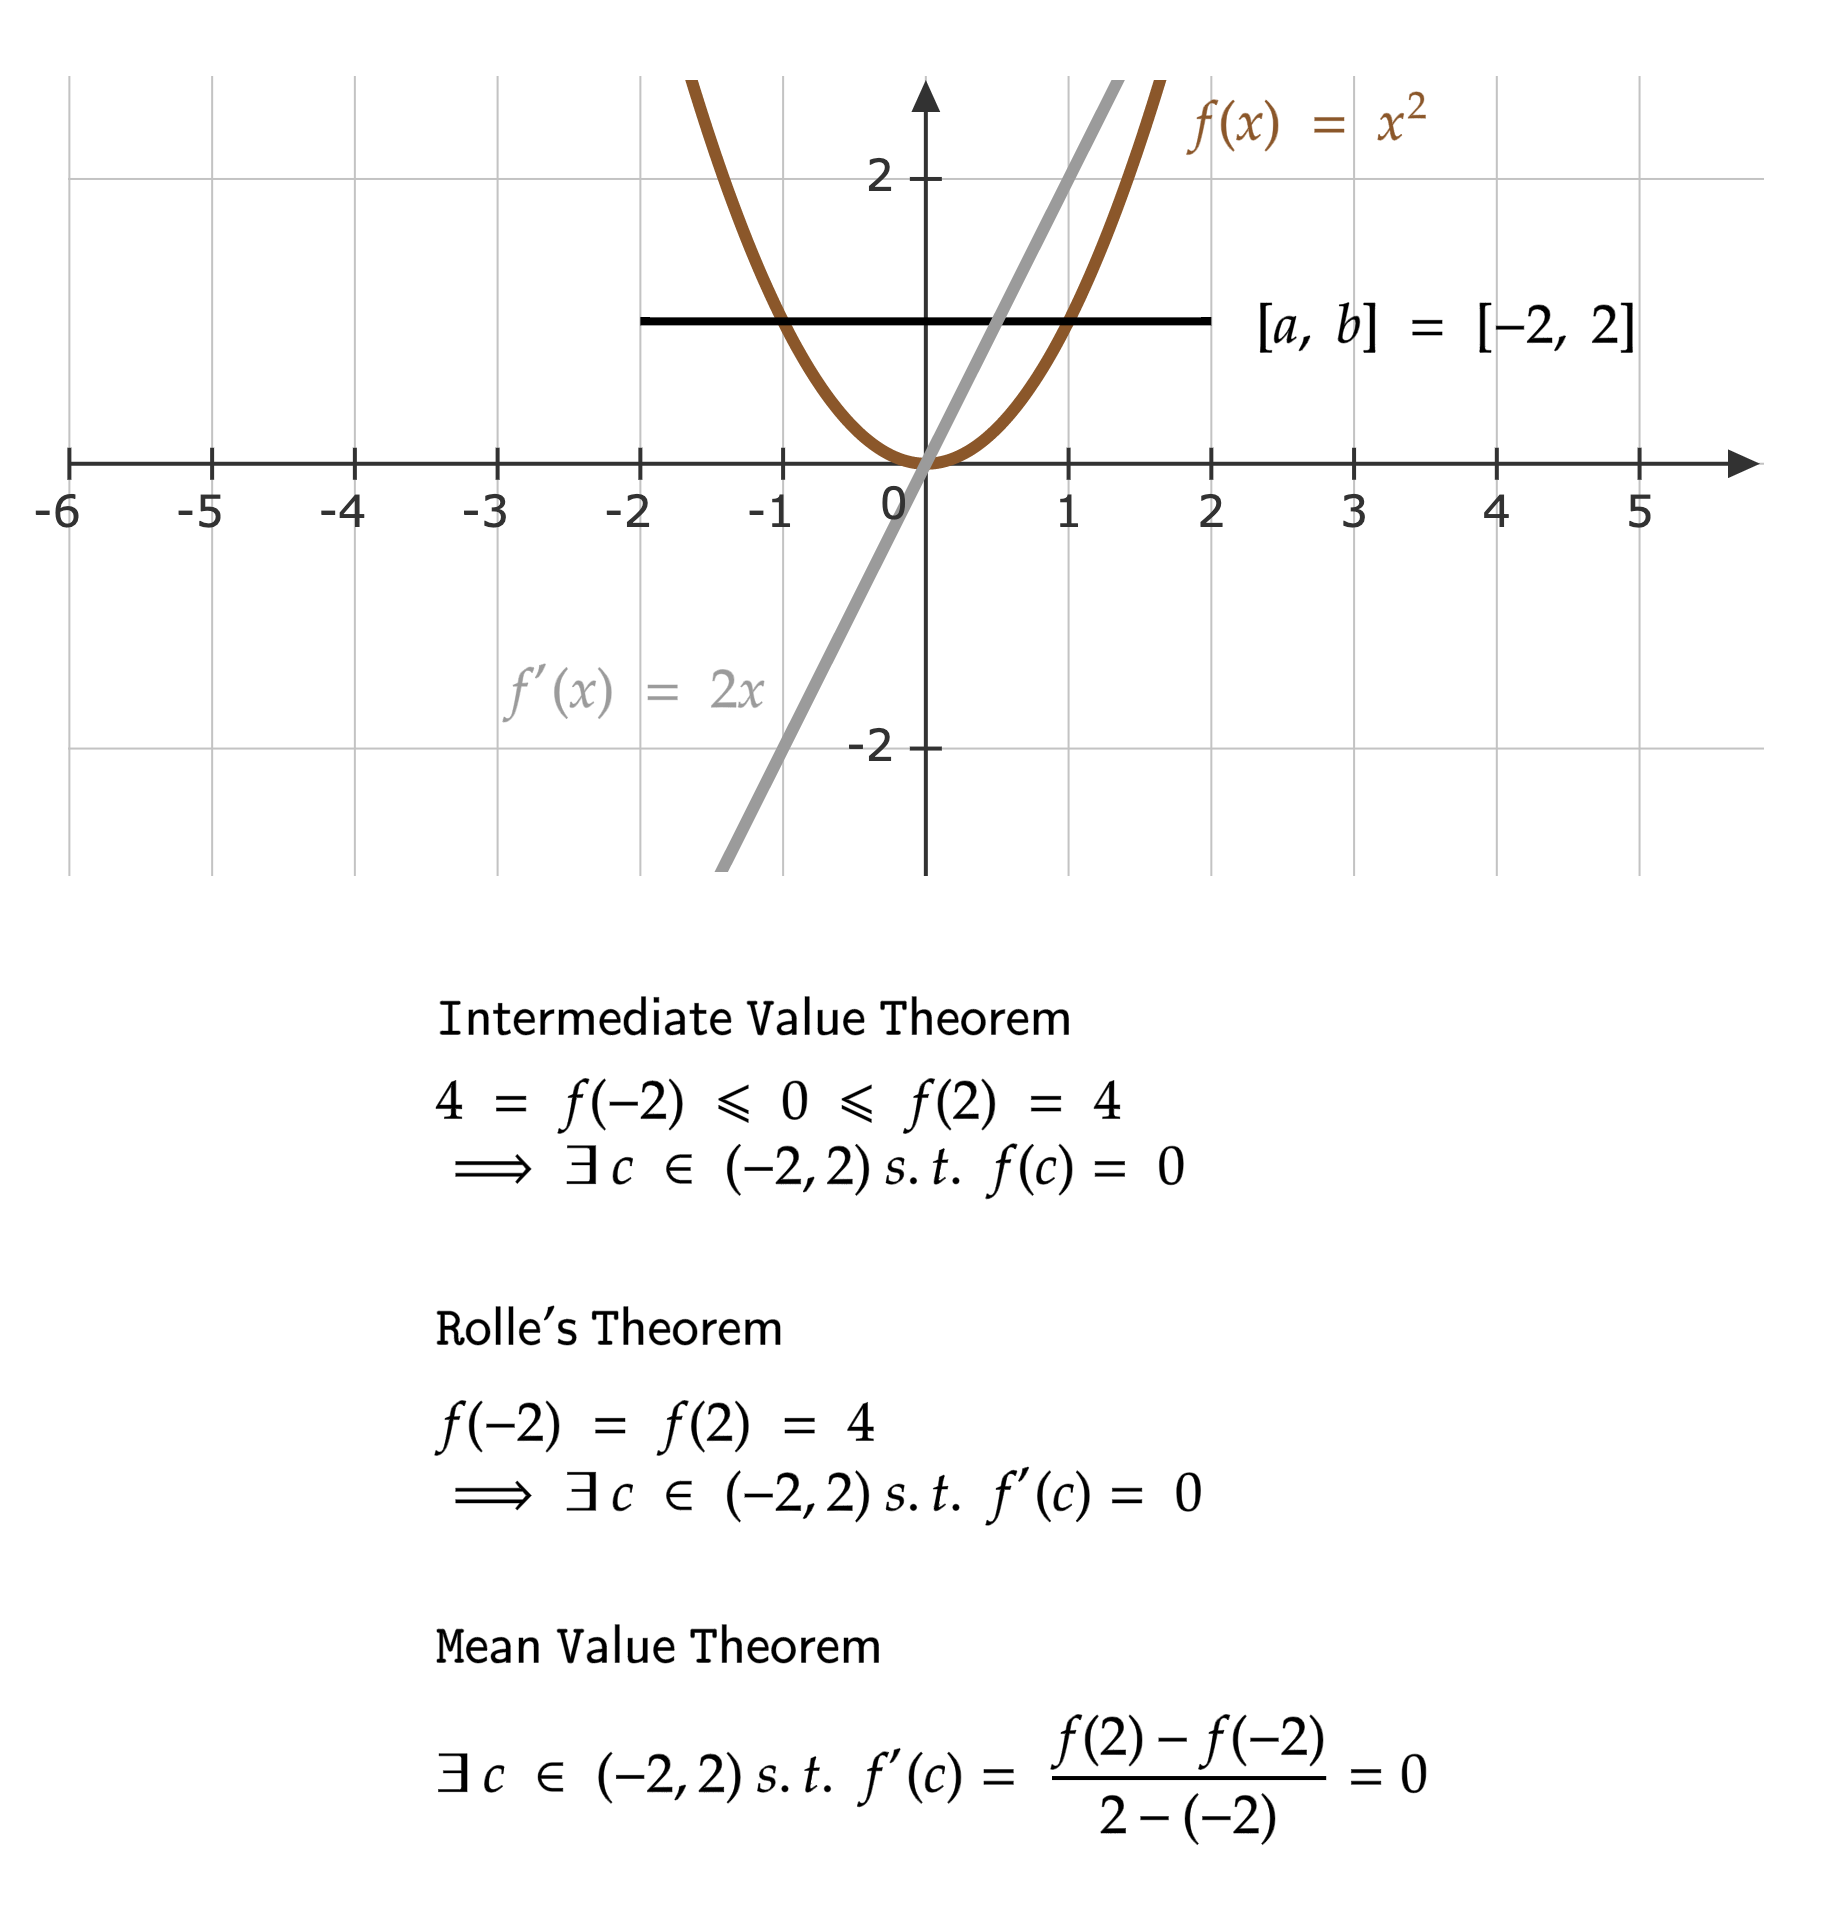
\includegraphics[width=\textwidth]{figures/fig-7b.png}
\end{center}
\end{ex}

\begin{marginfigure}
Common Taylor Series include,
\begin{align*}
    &\sin x=\sum_{n=0}^{\infty} \frac{(-1)^n}{(2 n+1) !} x^{2 n+1} \\
    &\LineBreak \\
    &\cos x=\sum_{n=0}^{\infty} \frac{(-1)^n}{(2 n) !} x^{2 n} \\
    &\LineBreak \\
    &e^x=\sum_{n=0}^{\infty} \frac{x^n}{n !} \\
    &\LineBreak \\
    &(1+x)^k=\sum_{n=0}^{\infty}\binom{n}{k} x^n \\
    &\LineBreak \\
    &\frac{1}{1-x}=\sum_{k=0}^{\infty} x^k \quad |x| < 1 \\
    &\LineBreak \\
    &\log (1+x)=\sum_{k=0}^{\infty} \frac{(-1)^k x^{k+1}}{k+1} \quad |x| < 1
\end{align*}
\end{marginfigure}

\begin{thm}[Taylor's Theorem]
    Suppose $f \in C^n([a, b])$ and $f^{(n+1)}$ exists on the interval $[a, b]$. Let $x_0 \in [a, b]$. Then $\forall x \in[a, b]$,
    \[\exists \xi(x) \in (x_0, x) \text{ s.t. } f(x)=P_n(x)+R_n(x)\]
    where,
    \begin{align*}
    &P_n(x) =\sum_{k=0}^n \frac{f^{(k)}\left(x_0\right)}{k !}\left(x-x_0\right)^k \\
    &R_n(x)=\frac{f^{(n+1)}(\xi(x))}{(n+1) !}\left(x-x_0\right)^{n+1}
    \end{align*}    
\end{thm}

\begin{rmk}
    $P_n(x)$ is called the \textbf{$n$th Taylor polynomial} for $f$ about $x_0$, and $R_n(x)$ is called the \textbf{truncation error} associated with $P_n(x)$.
\end{rmk}

\begin{ex}{Taylor Polynomials and Error Bounds}{label}
To find the second Taylor polynomial of,
\[g(x) = \sqrt{1 + x} - 1\]
about $x_0 = 0$,
\begin{enumerate}
    \item $g(x) = (1 + x)^{1/2} - 1$ and $g(0) = 0$
    \item $g^{\prime}(x) = \frac{1}{2}(1 + x)^{-1/2}$ and $g^{\prime}(0) = \frac{1}{2}$
    \item $g^{\prime\prime}(x) = -\frac{1}{4}(1 + x)^{-3/2}$ and $g^{\prime\prime}(0) = -\frac{1}{4}$
    \item $g^{\prime\prime\prime}(x) = \frac{3}{8}(1 + x)^{-5/2}$ and $|g^{\prime\prime\prime}(\xi(x))| = \frac{3}{8} \cdot \frac{1}{|1 + \xi(x)|^{\frac{5}{2}}} \leq \frac{3}{8}$
\end{enumerate}
Thus, $P_2(x) = \frac{x}{2} - \frac{x^2}{8}$ with the error,
\[|g(x) - P_2(x)| = |R_2(x)| \leq \frac{1}{16}\]
In comparison, we can approximate $g(0.0001)$ using $P_2(0.001)$ with 5-digit truncation. This gives a relative error of $\approx 0.001 \%$.
\end{ex}

\begin{rmk}
    It is sometimes easier to use Taylor series expansion when asked to compute the $n$-th Taylor polynomial for a function $f$.
\end{rmk}

\subsection{Convergence Order}
\begin{defn}[$Q$-Convergence]
    \sloppy A sequence $\{\mathbf{x}_k\}_k$ in $\R^n$ converges to $\mathbf{x}^* \in \R^n$ if $\|\mathbf{x}_k - \mathbf{x}^*\| \rightarrow 0$ as $k \rightarrow \infty$. Suppose $\mathbf{x}_k \neq \mathbf{x}^*$ for sufficiently large $k$. Then $\{\mathbf{x}_k\}_k$ converges to $\mathbf{x}^*$ at \textbf{order} $p$ with an asymptotic error constant $C > 0$ whenever,
    \[\lim_{k \rightarrow \infty} \frac{\|\mathbf{x}_{k+1} - \mathbf{x}^*\|}{\|\mathbf{x}_k - \mathbf{x}^*\|^p}  = C\]
    By convention, we have the following,
    \begin{itemize}
        \item If $p = 1$, the converge is called \textbf{$Q$-linear}
        \item If $p = 2$, the converge is called \textbf{$Q$-quadratic}
        \item If $p > 1$, the converge is called \textbf{$Q$-superlinear}
    \end{itemize}
\end{defn}


\begin{ex}{The Significance of $p$}{label}
    Suppose $\mathbf{x}_k$ converges to $\mathbf{x}^*$ with order $p$. There exists \text{$r \in (0, 1)$} and constants \text{$C_1, C_2 > 0$} so that for \text{$p = 1$} and \text{$p > 2$},
    \begin{enumerate}
        \item The error is reduced by a factor of $r$ between $\mathbf{x}_k$ and $\mathbf{x}_{k+1}$
        \[(Linear) \quad C_1 \cdot r^k \leq \|\mathbf{x}_k - \mathbf{x}^* \| \leq C_2 \cdot  r^k\]
        \item The error is reduced by a factor of $r^{p^k}$ between $\mathbf{x}_k$ and $\mathbf{x}_{k+1}$
        \[(Superlinear) \quad C_1 \cdot  r^{p^k} \leq \|\mathbf{x}_k - \mathbf{x}^* \| \leq C_2 \cdot r^{p^k}\]
    \end{enumerate}
    Moreover, the order $p$ is unique. 
\end{ex}

\begin{rmk}
\sloppy Suppose $\mathbf{x}_k$ converges to $\mathbf{x}^*$ with order $p$ and A.E.C $C > 0$. It was left as an exercise to prove that,
    \begin{equation}
    \lim _{k \rightarrow \infty} \frac{\left\|\mathbf{x}_{k+1}-\mathbf{x}^*\right\|}{\left\|\mathbf{x}_k-\mathbf{x}^*\right\|^q}=\left\{\begin{array}{c}
    0, \text { if } q<p \\
    C, \text { if } q=p \\
    \infty, \text { if } q>p
    \end{array}\right.
    \end{equation}
    
\end{rmk}
\begin{marginfigure}
     The improvement in digits per iteration depends on the convergence order,
     \begin{enumerate}
         \item In the linear case, the digit improvement rate is constant
         \item In the quadratic case, the digit improvement rate doubles
         \item In the superlinear case, the digit improvement rate increases
     \end{enumerate}
\end{marginfigure}

\begin{ex}{Convergence Order}{label}
    The following sequences $\{x_k\}_k$ converge to zero,
    \begin{enumerate}
        \item $x_k := 2^{-i}$ is linear with A.E.C = $\frac{1}{2}$
        \item $x_k := 2^{-2i+1}$ is linear with A.E.C = $\frac{1}{4}$
        \item $x_k := 2^{-2^i}$ is quadratic with A.E.C = $1$
    \end{enumerate}
\end{ex}

\noindent The notion of $Q$-convergence may be insufficient to describe a sequence when the limit does not exist. We require a weaker notion,

\begin{defn}[$R$-Linear Convergence]
    \sloppy Let $\{\mathbf{x}_k\}_k$ be a sequence that converges to \text{$\mathbf{x}^* \in \R^n$}.
    We say that $\{\mathbf{x}_k\}$ converges \textbf{$R$-linearly} if there is a non-negative real sequence \text{$\{a_k\}^{\infty}_{k=0} \subset \R$} converging $Q$-linearly to zero so that for sufficiently large $k$,
    \[\|\mathbf{x}_k - \mathbf{x}^*\| \leq a_k\]
\end{defn}

\noindent Given $f: \R^n \rightarrow \R^n$, we are often required to find solutions,
\[\mathbf{x} \in \R^n \text{ such that } f(\mathbf{x}) = \mathbf{0}\]
\begin{ex}{Nonlinear Equations with Known Solutions}{label}
\begin{enumerate}
    \item $f(x) = ax^2 + bx + c$ is solved using the quadratic formula
    \item $f(x) = x - e^{-x}$ is solved using the Lambert $W$ function
\end{enumerate}
\end{ex}

\begin{marginfigure}
    To use the Lambert $W$ function, remark that $y = xe^x$ if and only if $W(y) = x$.
\end{marginfigure}

\noindent In general, nonlinear systems of equations may have one, two, or even infinitely-many roots. We want to develop a method for approximating these roots by rapidly converging sequences of points. 

\subsection{Bisection Method}
We will make use of the following fact,

\begin{lem}
    Suppose $f \in C([a, b])$ and,
    \[\text{sign}(f(a)) \neq \text{sign}(f(b))\]
    then $\exists \xi \in (a, b)$ satisfying $f(\xi) = 0$.
\end{lem}

\noindent The basic idea of the \textbf{bisection method} is to,
\begin{enumerate}
    \item Assume that $\text{sign}(f(a)) \neq \text{sign}(f(b))$ on the interval $[a,b]$
    \item Define a variable for the midpoint of the interval, $m = a+b/2$
    \item If $\text{sign}(f(a)) \neq \text{sign}(f(m))$, consider the new interval $[a, m]$
    \item Otherwise, consider the interval $[m, b]$
    \item Repeat the previous steps until the interval length is small.
\end{enumerate}

\begin{rmk}
    The bisection method will return a root, if one exists, but it will not specify which root it has returned.
\end{rmk}

\begin{algorithm}
	  \caption{The Bisection Method}\label{bisection}
	  \Function{bisection($a, b, \texttt{tol}$)}{
	            \Comment{Assume $f$ is defined}
	    		\Comment{and that sign$(f(a)) \neq$ sign$(f(b))$}
	    \While{$b-a > \texttt{tol}$}{
	    		$m \assign (a+b)/2$\;
		    	\If{$\text{sign}(f(a)) \neq \text{sign}(f(b))$}{
		    	$b \assign m$\;
		      }
		    	\Else{
		    	  $a \assign m$\;
		     	}
	     	}
	    \Return{$m$}\;
	  }
\end{algorithm}

\noindent We want to know \textbf{how quickly the bisection method converges}. 

\begin{thm}
    The number of iterations $k$ to reach an accuracy of $\epsilon$ is,
    \[\frac{\log \left(b-a\right) - \log \epsilon}{\log 2} \leq k\]
    using the bisection method.
\end{thm}

\begin{proof}
We will use the following notation,
\begin{enumerate}
    \item $a_k$ and $b_k$ are the left and right endpoints of the $k$-th interval
    \item $x_k$ is the midpoint of the interval $[a_k, b_k]$
\end{enumerate}
Observe that,
\[\left|x^*-x_k\right| \leq b_k-a_k \leq \frac{1}{2}\left(b_{k-1}-a_{k-1}\right)\]
By iterating the recurrence, we obtain that,
\[\left|x^*-x_k\right| \leq \left(\frac{1}{2}\right)^k\left(b_0-a_0\right)=\underbrace{\frac{b-a}{2^k}}_{\mathbf{a}_k}\]
Since $\{\mathbf{a}_k\}$ converges $Q$-linearly to zero, the bisection method converges $R$-linearly. Using the monotonicity of the logarithm function,
\[\frac{b-a}{2^k} \leq \epsilon \iff \frac{b-a}{\epsilon} \leq 2^k\]
implies that,
\[\frac{\log \left(\frac{b-a}{\epsilon}\right)}{\log 2} \leq k \iff \frac{\log \left(b-a\right) - \log \epsilon}{\log 2} \leq k\]
\end{proof}


\subsection{Fixed Point Iteration}
\begin{defn}[Fixed Point]
    A point $x^* \in \R$ is a \textbf{fixed point} for a function $g: \R \rightarrow \R$ if the condition $g(x^*) = x^*$ holds.
\end{defn}

\noindent Fixed points and roots of functions can be related as follows.
\begin{enumerate}
    \item If $x^*$ is a root of $f$, then $x^*$ is a fixed point of $g(x) := x + f(x)$.
    \item If $x^*$ is a fixed point of $g$, then $x^*$ is a root of $f(x) := g(x) - x$
\end{enumerate}

\begin{marginfigure}
    Note that there are many other choices for relating $g(x)$ and $f(x)$.
\end{marginfigure}

\begin{thm}[Fixed Point Theorem]
    Suppose $g \in C([a, b])$.
    \begin{enumerate}
        \item If $a \leq g(x) \leq b$ for all $x \in [a, b]$, then $g$ has a fixed point,
        \[x^* \in [a, b]\]
        \item If $g$ is differentiable on $(a, b)$ and $\exists L \in (0, 1)$ so that,
        \[|g^{\prime}(x)| \leq L\]
        for all $x \in (a, b)$, then there is at most one fixed point in $[a, b]$
    \end{enumerate}
\end{thm}

\begin{proof}
    We will prove each claim in turn. 
    \begin{enumerate}
        \item \textbf{(Existence)} Suppose $g(a) = a$ or $g(b) = b$. Then $a$ or $b$ is a fixed point of $g$. Otherwise, $a < g(a) < b$ since $a \leq g(x) \leq b$ by assumption. Define a function $f(x) := x - g(x)$. We know that $f(a) = a - g(a) < 0$ and $f(b) = b - g(b) > 0$. By the Intermediate Value Theorem, there exists $\xi \in(a, b)$ so that $f(\xi) = 0$. That is, $\xi = g(\xi)$ is a fixed point of $g$. 
        \item \textbf{(Uniqueness)} Suppose $g$ is differentiable on $(a, b)$ and $\exists L \in (0, 1)$ so that $|g^{\prime}(x)| \leq L$. Assume that $x^*, y^* \in [a, b]$ are fixed points. By the Mean Value Theorem, there exists $\xi \in (x^*, y^*)$ such that,
        \[\left|g^{\prime}(\xi)\right|=\left|\frac{g(y^*)-g(x^*)}{y^*-x^*}\right|=\left|\frac{y^*-x^*}{y^*-x^*}\right|=1\]
        This contradicts that $\left|g^{\prime}(x)\right| \leq L<1$ for all $x \in (a, b)$.
    \end{enumerate}
\end{proof}

\begin{marginfigure}
Visualization of the existence criteria for the fixed point theorem.
\begin{center}
       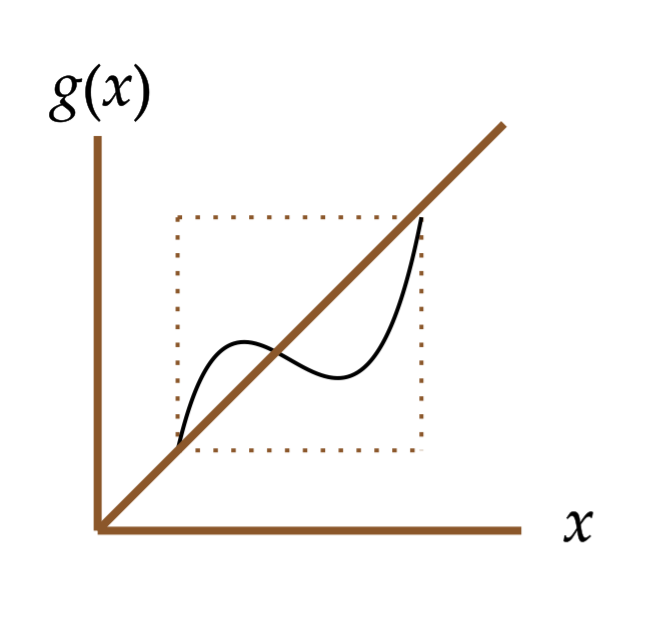
\includegraphics[width=0.8\textwidth]{figures/fig-2.png}
\end{center}
\end{marginfigure}

\begin{defn}[Fixed Point Iteration]
    Let $x_0 \in [a, b]$. The \textbf{fixed point iteration sequence} is the sequence defined inductively by,
    \begin{align*}
    x_1 &=g\left(x_0\right) \\
    x_2 &=g\left(x_1\right)=g\left(g\left(x_0\right)\right) \\
    & \vdots \\
    x_k &=g(x_{k-1}) = \underbrace{g\left(\ldots\left(g\left(x_0\right)\right) \ldots\right)}_{k \text { times }}
    \end{align*}
\end{defn}

\noindent We will establish conditions for the convergence of the fixed point iteration sequence in the theorem that follows.

\begin{thm}[Fixed Point Iteration Theorem]
    Suppose $g$ satisfies the hypothesis of the Fixed Point Theorem with a unique fixed point $x^*$.
    \begin{enumerate}
        \item $\left|x_k-x^*\right| \leq L^k \cdot \left|x_0-x^*\right|$
        \item $\left|x_k-x^*\right| \leq L^k \cdot \max \left\{\left|x_0-a\right|,\left|x_0-b\right|\right\}$
    \end{enumerate}
    for $0 \leq L < 1$ and $\{x_k\}$ defined as the fixed point iteration sequence. Observe that (1) states that $x_k$ converges $R$-linearly to $x^*$.
\end{thm}

\begin{proof}
    To prove (1),
    \[\left|x_k-x^*\right|=\left|g\left(x_{k-1}\right)-g\left(x^*\right)\right|\]
    by definition of $\{x_k\}$ and the fact that $x^* = g(x^*)$. By the Mean Value Theorem, there exists $\xi \in (x_{k-1}, x^*)$ such that,
    \begin{align*}
\left|x_k-x^*\right| &=\left|g\left(x_{k-1}\right)-g\left(x^*\right)\right| \\
&=\left|g^{\prime}\left(\xi_{k-1}\right)\right|\left|x_{k-1}-x^*\right| \\
&\leq L|x_{k-1} - x^*|
\end{align*}
Iterating the recurrence gives that,
\[|x_k - x^*| \leq L^k\left|x_0-x^*\right| \rightarrow 0 \text { as } k \rightarrow \infty\]
To prove (2), we use that,
\[|x_0 - x^*| \leq \max \left\{\left|x_0-a\right|,\left|x_0-b\right|\right\}\]
because $x_0$ and $x^*$ are in the interval $[a,b]$.
\end{proof}

\begin{algorithm}
	  \caption{Fixed Point Iteration}\label{fpi}
	  \Function{FPI($a, b, \texttt{tol}$)}{
	            \Comment{Assume $g$ is defined and that it satisfies the fixed point theorem hypothesis}
	    $x \assign x_0$\;
	    $x^{\prime} \assign g(x)$\;
	    \While{$|x^{\prime} - x| > \texttt{tol}$}{
	    		$x \assign x^{\prime}$\;
	    		$x^{\prime} \assign g(x)$\;
	    } \Return{$x^{\prime}$}\;
	  }
\end{algorithm}

\begin{marginfigure}
We could have used,
\begin{align*}
&\frac{\left|x_k-x_{k-1}\right|}{\left|x_k\right|}< \texttt{tol} \\
&\left|x_k-g\left(x_k\right)\right|<\texttt{tol}
\end{align*}
as our stopping criteria.
\end{marginfigure}

\begin{ex}{Finding the root of $f(x) = x - e^{-x}$}{label}
    \begin{center}
       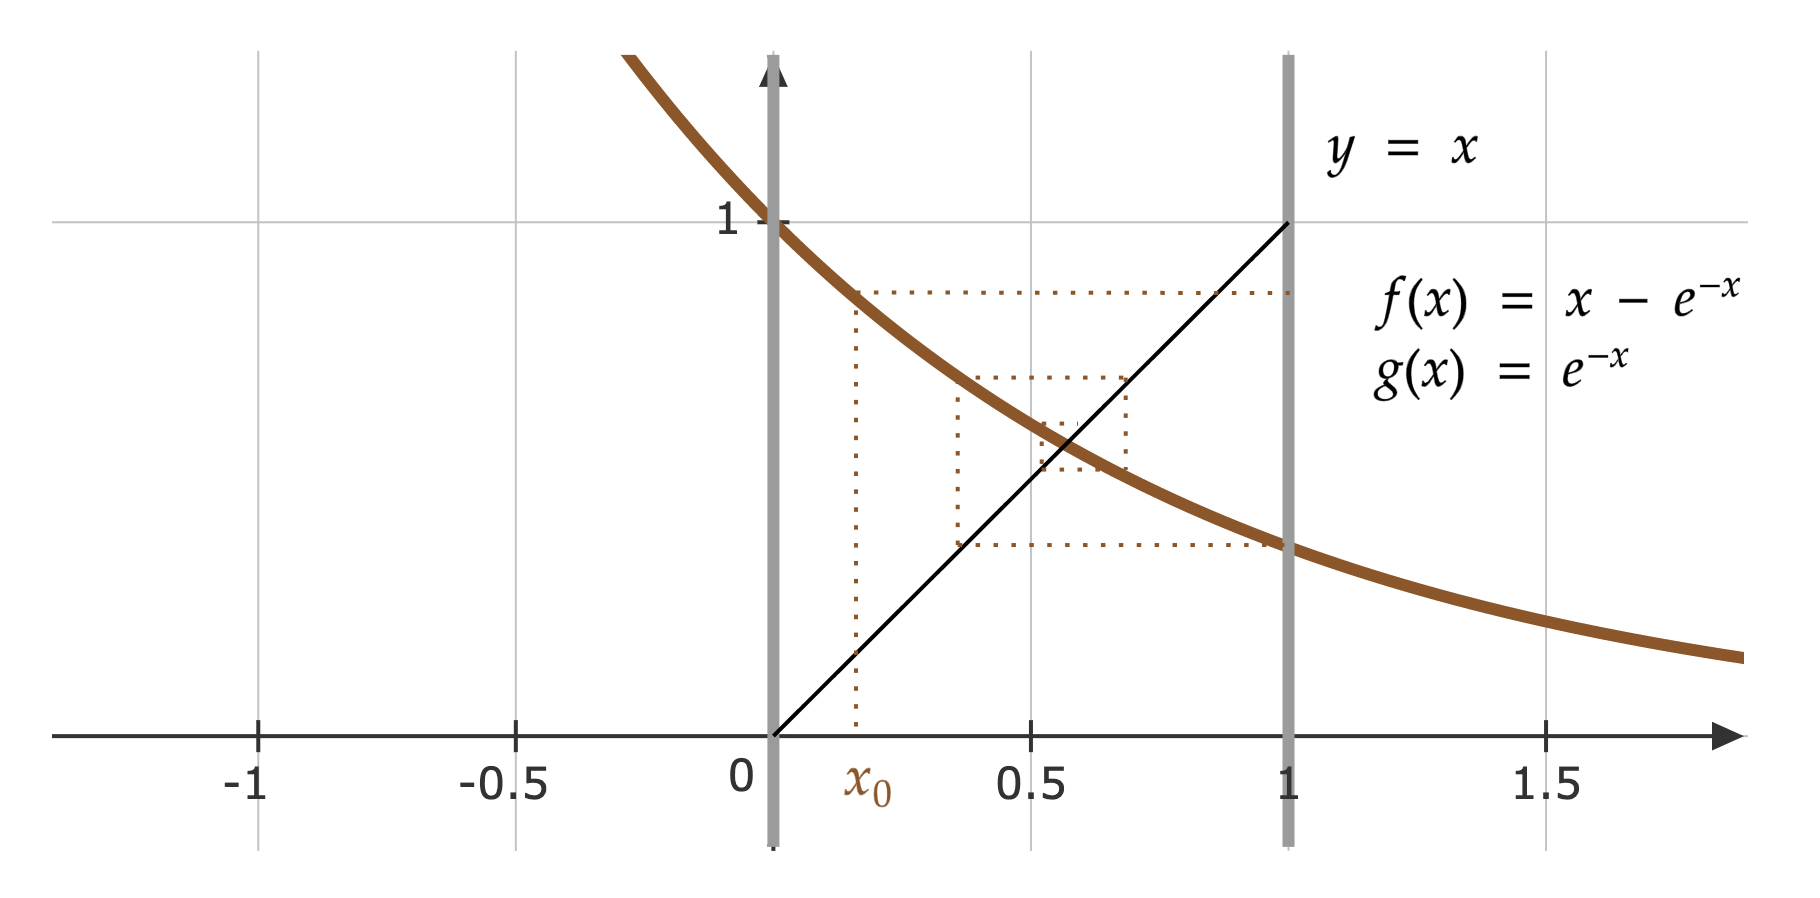
\includegraphics[width=\textwidth]{figures/fig-8.png}
\end{center}
\end{ex}

\noindent We want to know \textbf{how quickly the fixed point method converges}. 

\begin{thm}
    Under the following conditions,
    \begin{enumerate}
        \item $g$ satisfies the hypothesis of the Fixed Point Theorem
        \item $g^{\prime} \in C([a, b])$ with $g^{\prime}(x^*) \neq 0$
    \end{enumerate}
    Then, $\{x_k\}_k$ converges $Q$-linearly with A.E.C $ |g^{\prime}(x^*)|$.
\end{thm}

\begin{proof}
    Since $x^{*} = g(x^{*})$ and $x_{k+1} = g(x_k)$, then by the Mean Value Theorem $\exists \xi_k \in (x_k, x^*)$ such that,
    \[\left|x_{k+1}-x^*\right|=\left|g\left(x_k\right)-g\left(x^*\right)\right|=\left|g^{\prime}\left(\xi_k\right)\right|\left|x_k-x^*\right|\]
    by the Mean Value Theorem. Taking $k \rightarrow \infty$, we obtain $x_k \rightarrow x^*$ and $\xi_k \rightarrow x^*$. By the continuity of $g^{\prime}$, we conclude that,
    \[\lim _{k \rightarrow \infty} \frac{\left|x_{k+1}-x^*\right|}{\left|x_k-x^*\right|}=\lim _{k \rightarrow \infty}\left|g^{\prime}\left(\xi_k\right)\right|=\left|g^{\prime}\left(x^*\right)\right|\]
    with  $0 < \left|g^{\prime}\left(x^*\right)\right| < 1$ implying $Q$-linear convergence.
\end{proof}

\begin{marginfigure}
    The continuity of $g^{\prime}$ justifies us in bringing the limit inside.
\end{marginfigure}

\begin{rmk}
    If $g^{\prime}(x^*) = 0$, then the fixed point iteration might converge faster than linearly because a smaller A.E.C. gives faster convergence.
\end{rmk}

\begin{thm}
   Suppose $g \in C^p([a, b])$ has a fixed point $x^*$. If the fixed point iteration of $g$ converges,  $g^{(i)}\left(x^*\right)=0$ for all $i \in [p-1]$, and $g^{(p)}\left(x^*\right) \neq 0$, then the fixed point iteration converges at order $p$.
\end{thm}

\begin{proof}
   This is left as an exercise on Assignment 1.
\end{proof}

\subsection{Newton's Method}
Previously, we saw that,
\begin{enumerate}
    \item $g^{\prime}(x^*) \neq 0 \implies$ fixed point iteration converges linearly
    \item $g^{\prime}(x^*) = 0 \implies$ fixed point iteration may converge at higher order
\end{enumerate}

\begin{marginfigure}
    If $f^{\prime}\left(x^*\right)=0$, then Newton's Method is undefined or converges linearly.
\end{marginfigure}

\noindent The goal of \textbf{Newton's Method} is to construct a fixed point function $g$ to find a root of $f$ at quadratic order. To do this, we define,
\[g(x) = x + \phi(x) f(x)\]
for some unknown function $\phi(x)$. This ensures that,
\[f\left(x^*\right)=0 \implies g\left(x^*\right)=x^*\]
We require that $g^{\prime}(x^*) = 0$ whenever $f(x^*) = 0$ for the fixed point iteration to be of quadratic order. This is equivalent to,
\[0=g^{\prime}\left(x^*\right)=1+\phi^{\prime}\left(x^*\right) \underbrace{f\left(x^*\right)}_{=0}+\phi\left(x^*\right) f^{\prime}\left(x^*\right)\]
which suggests that $\phi$ is of the form,
\[\phi\left(x^*\right)=-\frac{1}{f^{\prime}\left(x^*\right)}\]
with the fixed point function,
\[g(x)=x-\frac{f(x)}{f^{\prime}(x)}\]

\noindent Therefore, we define the fixed point iteration,
\[x_{k+1}=x_k-\frac{f\left(x_k\right)}{f^{\prime}\left(x_k\right)}\]
given some $x_0$ chosen in advance.

\begin{ex}{Recovering the Babylonian Sequence}{label}
    Given \text{$a > 0$}, we can compute $\sqrt{a}$ using Newton's method and
    \begin{align*}
        f(x) &= x^2 - a \\
        f^{\prime}(x) &= 2 x
    \end{align*}
    We will iterate the recurrence,
    \[x_{k+1}=x_k-\frac{x_k^2-a}{2 x_k}\]
    to recover the Babylonian sequence.
\end{ex}

\begin{marginfigure}
    Newton's Method is not guaranteed to converge for every choice of $x_0 \in [a, b]$.
\end{marginfigure}

\noindent The following theorem establishes that Newton's Method will converge if the initial choice $x_0$ is sufficiently close to $x^*$.

\begin{thm}[Local Convergence Theorem]
   Let $f \in C^2{[a,b]}$ and $x^* \in [a, b]$ be a root of $f$ with $f^{\prime}(x^*) \neq 0$. There exists $\delta > 0$ such that Newton's Method converges quadratically $\forall x_0 \in\left[x^*-\delta, x^*+\delta\right]$.
\end{thm}

\noindent We can \textbf{generalize Newton's method} to functions in $n$ variables,
\begin{align*}
x_k &\rightarrow \mathbf{x}_k \\
f\left(x_k\right) &\rightarrow f\left(\mathbf{x}_k\right) \\
f^{\prime}\left(x_k\right) &\rightarrow J_f\left(\mathbf{x}_k\right)
\end{align*}
where $J_f$ is the \textbf{Jacobian matrix}. Recall that,
\[J_{\mathbf{f}}(\mathbf{x})=\left(\begin{array}{ccc}
\frac{\partial f_1}{\partial x_1}(\mathbf{x}) & \ldots & \frac{\partial f_1}{\partial x_n}(\mathbf{x}) \\
\vdots & \ddots & \vdots \\
\frac{\partial f_n}{\partial x_1}(\mathbf{x}) & \ldots & \frac{\partial f_n}{\partial x_n}(\mathbf{x})
\end{array}\right) \quad \text{ for } \quad f(x)=\left(\begin{array}{c}
f_1(\mathbf{x}) \\
\vdots \\
f_n(\mathbf{x})
\end{array}\right)\]
\noindent We select $\mathbf{x}_0$ in advance, and then we iterate as follows,
\[J_{\mathbf{f}}\left(\mathbf{x}_k\right)\left(\mathbf{x}_{k+1}-\mathbf{x}_k\right)=-\mathbf{f}\left(\mathbf{x}_k\right)\]
In practice, we can first solve for $\mathbf{s}_k:=\mathbf{x}_{k+1}-\mathbf{x}_k$ in,
\[J_{\mathbf{f}}\left(\mathbf{x}_k\right) \mathbf{s}_k=-\mathbf{f}\left(\mathbf{x}_k\right)\]
and then update $\mathbf{x}_{k+1}=\mathbf{x}_k+\mathbf{s}_k$.
\begin{marginfigure}
    Newton's method can be computationally intensive in higher dimensions because we must compute $O(n^2)$ derivatives per iteration.
\end{marginfigure}